\documentclass[10pt]{article}

\usepackage{notes}

\begin{document}

\section*{Complex Operations}
\label{sec:compops}

\subsection*{Addition}
\label{subsec:addition}

\subsubsection*{Algebraic Interpretation}
\label{subsubsec:algint}
Let $s,t,x,y \in \mathbb{R}$ and let $z,w \in \mathbb{C}$ such that  $z = (x,y) \text{ and } w = (s,t)$ then,
\[ z + w = (x+s, y+t) \]

We could also write:
\[ z + w = (x + yi) + (s + ti) = (x + s) + (y + t)i \] 

\redit{The above forms are equivalent.}

\subsubsection*{Geometric Interpretation}

The geometric form of complex number addition gives us a better intuition for what these numbers really mean. 

\begin{figure}[h!]
\begin{center}
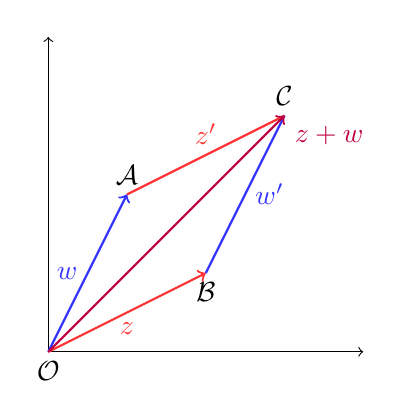
\begin{tikzpicture}
\draw (0,0) node[below]{$ \mathcal{O} $};
\draw [ <->] (0,4) node[left]{$ \ib $} -- (0,0) -- (4,0) node[below]{$ \rb $};
\draw [blue!80,thick,->] (0,0) -- (1,2) node[left,midway]{$ w $};
\draw (1,2) node[above]{$ \mathcal{A} $};
\draw [red!80,thick,->] (0,0) --(2,1) node[below,midway]{$ z $};
\draw (2,1) node[below]{$ \mathcal{B} $};
\draw [blue!80,thick] (2,1) -- (3,3) node[right,midway]{$ w' $};
\draw (3,3) node[above]{$ \mathcal{C} $};
\draw [red!80,thick] (1,2) -- (3,3) node[above,midway]{$ z' $}; 
\draw [thick,->,purple] (0,0) -- (3,3) node[below right]{$ z + w $};
\end{tikzpicture}
\caption{Addition over Complex Numbers}
\end{center}
\end{figure}

\begin{eqnarray*}
z = (x, y) = x + yi \\
w = (s, t) = s + ti \\
v = z + w = (x + s) + (y + t)i \\
\end{eqnarray*}


\textcolor{red}{Notice:} \\
We have constructed a parallelogram $\mathcal{O}ACB$ with vertices $O, A, B, C$ where $C$ is the point created by adding points $A$ and $B$ component-wise.

We have also constructed two congruent triangles $\Delta OAC$ and $\Delta OBC$ which share a hypotenuse $OC$ whose corresponding sides $OA$ and $BC$ as well as $AC$ and $OB$ are of equal length (respectively). The shared hypotenuse of these triangles ($OC$) has a length which is the sum of the lengths of $z$ and $w$.

\subsection*{Subtraction}
\label{subsec:subtract}
Subtraction of complex numbers is just a sign change for the number being subtracted.

\begin{figure}[h!]
\begin{center}
\begin{tikzpicture}
\draw [->] (0,0) -- (0,4) node[left]{$ \ib $};
\draw [<-] (0,-4) -- (0,0);
\draw [<-] (-4,0) -- (0,0);
\draw [->] (0,0) -- (4,0) node[below]{$ \rb $};
\draw [blue!80,thick,->] (0,0) -- (1,2) node[left,midway]{$ w $};
\draw [blue!80,thick,->] (0,0) -- (-1,-2) node[left,midway]{$ w' $};
\draw [orange!90,thick,->] (0,0) -- (1,-1) node[right]{$ u = z - w $};
\draw [red!80,thick,->] (0,0) --(2,1) node[below,midway]{$ z $};
\draw [orange!90,thick] (-1,-2) -- (1,-1);
\draw [orange!90,thick] (2,1) -- (1,-1);
\end{tikzpicture}
\caption{Subtraction over Complex Numbers}
\end{center}
\end{figure}

\subsubsection*{Algebraic Interpretation}

\subsubsection*{Geometric Interpretation}

\subsection*{Scalar Multiplication}
\label{subsec:scalar}
\subsubsection*{Algebraic Interpretation}

\subsubsection*{Geometric Interpretation}

\subsection*{Multiplication}
\label{subsec:mult}
\subsubsection*{Algebraic Interpretation}

\subsubsection*{Geometric Interpretation}

\subsection*{Conjugation}
\label{subsec:conj}
\subsubsection*{Algebraic Interpretation}

\subsubsection*{Geometric Interpretation}

\subsection*{Modulus}
\label{subsec:mod}
\subsubsection*{Algebraic Interpretation}

\subsubsection*{Geometric Interpretation}


\section*{Forms}
\label{sec:forms}

\subsection*{Cartesian}
\label{subsec:cart}

\subsection*{Polar}
\label{subsec:polar}

\subsection*{Euler}
\label{subsec:euler}

\section*{Proof Simplifications}
\label{sec:pf}

\section*{Solutions}
\label{sec:sol}


\subsection*{What does it mean to have an ``imaginary'' root?}
\label{subsec:root}


\subsection*{What does an ``imaginary'' root look like?}
\label{subsec:look}


\subsection*{Cubic Solutions}
\label{subsec:cubic}

\section*{Rotation by $i$}
\label{sec:rot}

\end{document}